\section{Overview of our Approach}\label{sec:walg}
\begin{figure*}[t]
   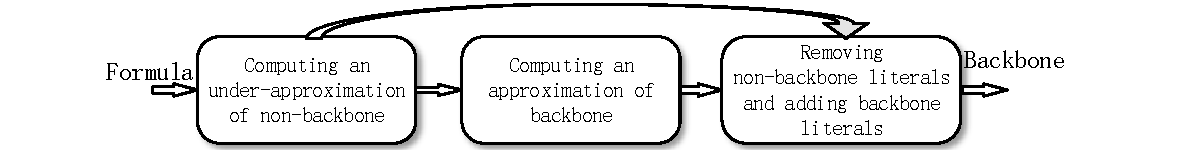
\includegraphics[scale=0.75]{Framework}
  \hspace*{-15mm} 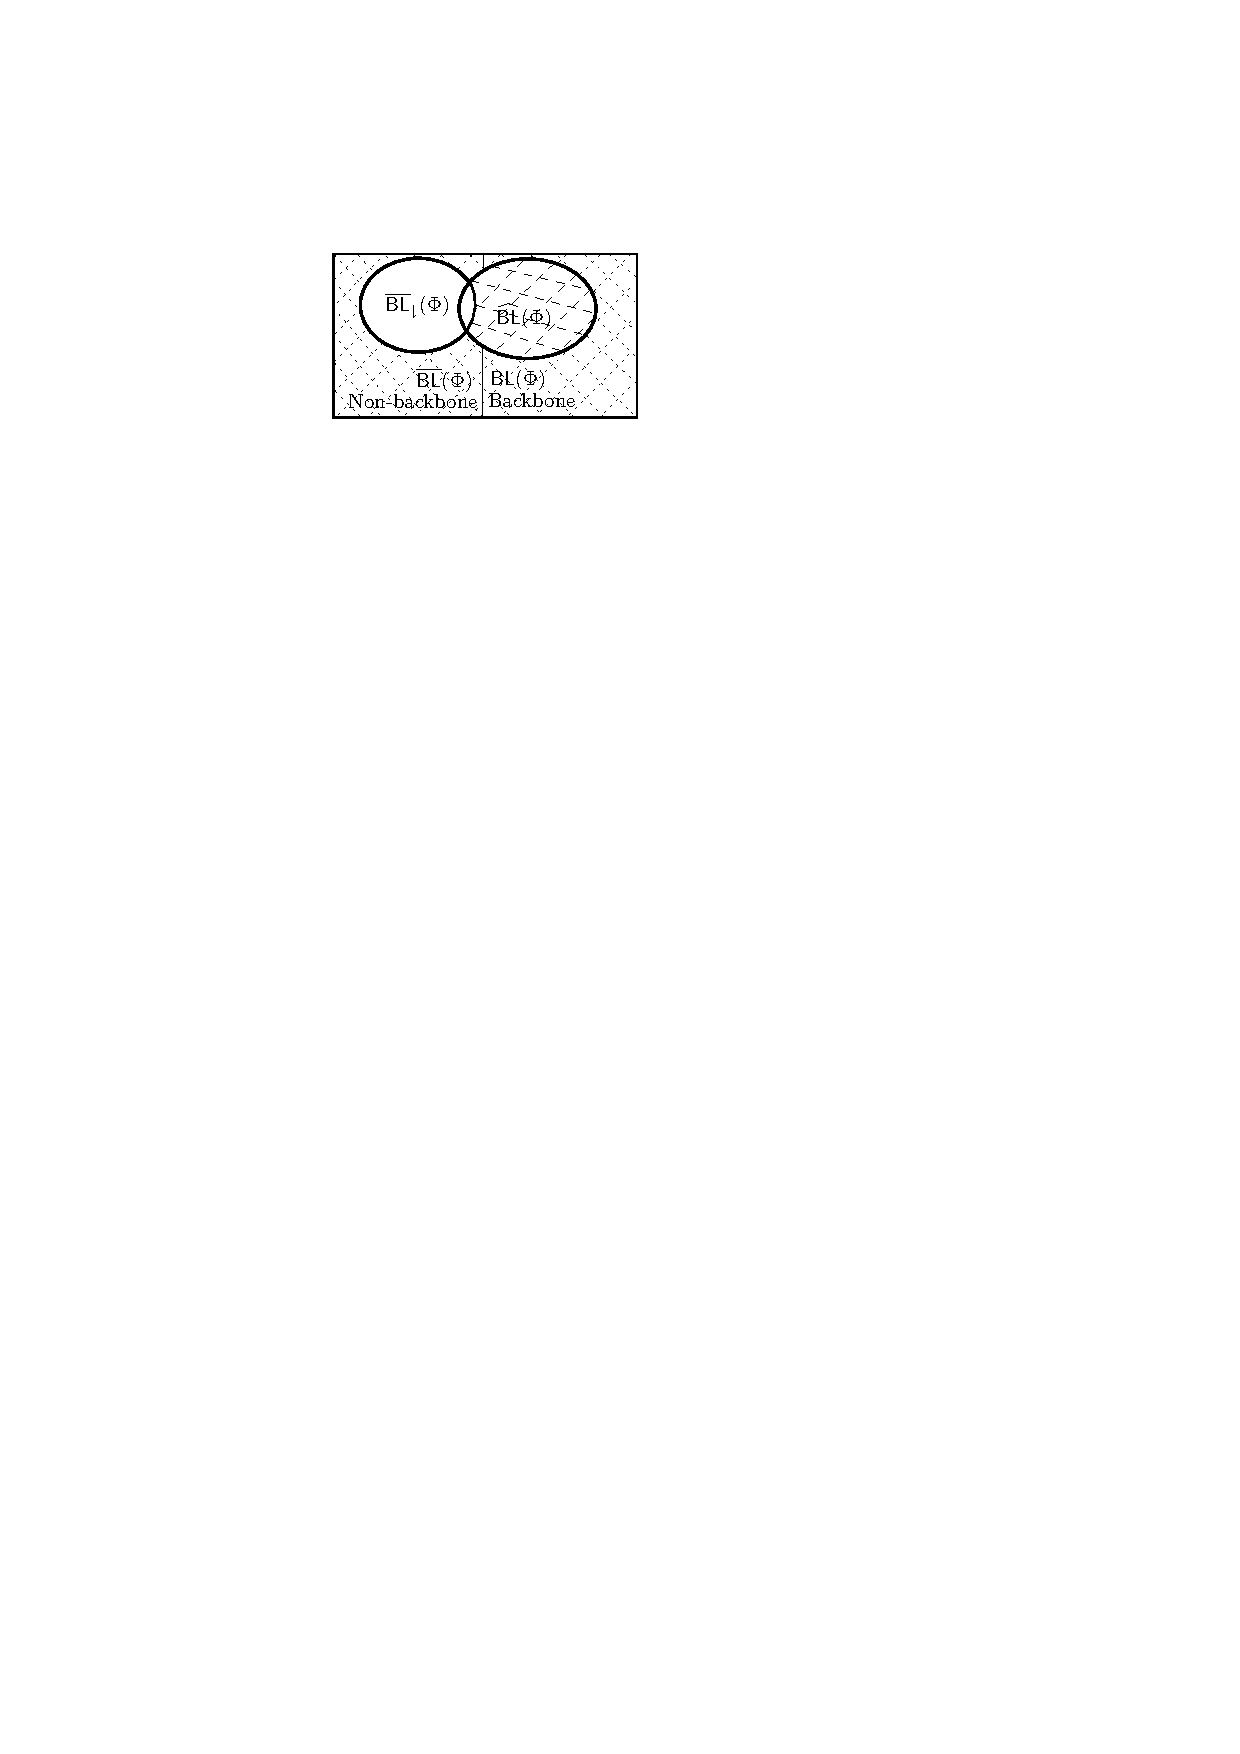
\includegraphics[scale=0.75]{Fig-backbone}
   \caption{Overview of our approach}
   \label{flow}
\end{figure*}

Figure \ref{flow} presents the overview of our approach \tool, which consists of three components. Taking a satisfiable formula
$\Phi$ as an input, \tool first computes an under-approximation $\NBLap(\Phi)\subseteq \NBL(\Phi)$ of the non-backbone of
$\Phi$. Then, \tool computes an approximation $\BLap(\Phi)$ of the backbone of $\Phi$ based on the set $\NBLap(\Phi)$, where each literal in $l\in \BLap(\Phi)$ has a high possibility to be a backbone literal of $\Phi$.
Finally, \tool removes non-backbone literals from $\BLap(\Phi)$ and adds backbone literals into $\BLap(\Phi)$ to compute the exact backbone of $\Phi$.

\medskip
\noindent{\bf Computing an under-approximation of non-backbone.}
Given a satisfiable formula $\Phi$, we first compute a model $\lambda$ of $\Phi$ by calling a SAT solver.
From the model $\lambda$, we compute a base under-approximation of non-backbone.
Later, we apply a Greedy-based algorithm to add more non-backbone literals into the base under-approximation, which results in the
under-approximation $\NBLap(\Phi)$.



\medskip
\noindent{\bf Computing an approximation of backbone.}
At this step, we apply an improved Whitening-based algorithm to compute the approximation $\BLap(\Phi)$.
The improved Whitening-based algorithm is an extension of the Whitening-based algorithm proposed by \cite{LMZ09} which
was used to compute \emph{frozen variables}, that are the variables whose values are fixed in a non-singleton set of models.
We use the Whitening-based algorithm of \cite{LMZ09} to compute the approximation $\BLap(\Phi)$ which is then refined by
a heuristic approach.


\medskip
\noindent{\bf Computing exact backbone.}
At this step, we use Algorithm 3 (Iterative algorithm) from \cite{JLM15} to compute backbone.
This algorithm uses SAT testing to check whether a literal is a backbone literal or not.
For instance, if $\Phi\vee \neg l$ is unsatisfiable but $\Phi$ is satisfiable, then $l$ must be a backbone literal of $\Phi$.


We first iteratively select one literal $l$ from $\BLap(\Phi)\setminus \NBLap(\Phi)$ such that $\lambda \models \neg l$ and test whether
$l$ is a backbone literal or not by checking the satisfiability of $\Phi\wedge l$ (dashed area in Figure \ref{flow}).
If $l$ is a backbone, we will add $l$ into $\Phi$ as a clause. Adding known backbone literals into $\Phi$ as clauses potentially speedups the later SAT testing \cite{JLM15,MPA2015}.
Then, we do the same testing for literals from $\Lit(\Phi)\setminus (\NBLap(\Phi)\cup\BLap(\Phi))$ (dotted area in Figure \ref{flow}).
After this step, the exact backbone and non-backbone are found.


In general, one can directly test all the literals to compute backbone without the two approximations.
However, the test heavily replies on SAT testing which may be time-cost.
Our approach makes two contributions compared to this na\"{\i}ve approach.
One is that we reduce the number of SAT calls using the known non-backbone literals $\BLap(\Phi)$.
The another one is that we first check literals that have high probability to be backbone literals so that backbone literals can be found as early as possible.

